%
% This is an example file and is hereby explicitly put in the
% public domain.
%
\documentclass[ppgc,diss,english]{iiufrgs}
% Para usar o modelo, deve-se informar o programa e o tipo de documento.
% Programas :
%   * cic       -- Graduação em Ciência da Computação
%   * ecp       -- Graduação em Ciência da Computação
%   * ppgc      -- Programa de Pós Graduação em Computação
%   * pgmigro   -- Programa de Pós Graduação em Microeletrônica
%
% Tipos de Documento:
%   * tc                -- Trabalhos de Conclusão (apenas cic e ecp)
%   * diss ou mestrado  -- Dissertações de Mestrado (ppgc e pgmicro)
%   * tese ou doutorado -- Teses de Doutorado (ppgc e pgmicro)
%   * ti                -- Trabalho Individual (ppgc e pgmicro)
%
% Outras Opções:
%   * english    -- para textos em inglês
%   * openright  -- Força início de capítulos em páginas ímpares (padrão da
%                   biblioteca)
%   * oneside    -- Desliga frente-e-verso
%   * nominatalocal -- Lê os dados da nominata do arquivo nominatalocal.def


% Use unicode
\usepackage[utf8]{inputenc}   % pacote para acentuação

% Necessário para incluir figuras
\usepackage{graphicx}           % pacote para importar figuras
\usepackage{tikz}

\usepackage{nicefrac}       % compact symbols for 1/2, etc.
\usepackage{amsfonts}       % blackboard math symbols
\usepackage{xspace}
\usepackage{amsmath}
\usepackage{amsthm}
\usepackage{amssymb}
\usepackage{algorithm}
\usepackage{algpseudocode}
\usepackage[capitalise]{cleveref}

% \usepackage{times}              % pacote para usar fonte Adobe Times
 \usepackage{palatino}
% \usepackage{mathptmx}          % p/ usar fonte Adobe Times nas fórmulas

\usepackage[alf,abnt-emphasize=bf]{abntex2cite}	% pacote para usar citações abnt

\providecommand{\multiset}[1]{\ensuremath{\{\!\!\{#1\}\!\!\}}}
\providecommand{\sas}{\ensuremath{\text{SAS}^{+}}\xspace}
\providecommand{\strips}{STRIPS\xspace}
\providecommand{\astar}{\ensuremath{\text{A}^{*}}\xspace}
\providecommand{\gbfs}{\ensuremath{\text{GBFS}}\xspace}
\providecommand{\wida}{\ensuremath{\text{W-IDA}^{*}}\xspace}
\providecommand{\ida}{\ensuremath{\text{IDA}^{*}}\xspace}
\providecommand{\hvalue}[1]{\ensuremath{h^{#1}}\xspace}
\providecommand{\hstarp}[1]{\ensuremath{h^*({#1})}\xspace}
\providecommand{\hff}{\hvalue{\text{FF}}}
\providecommand{\hgc}{\hvalue{\text{GC}}}
\providecommand{\hstar}{\hvalue{*}}
\providecommand{\hlmc}{\hvalue{\text{lm-c}}}
\providecommand{\hmax}{\hvalue{\text{max}}}
\providecommand{\hadd}{\hvalue{\text{add}}}
\providecommand{\h}{$h$\xspace}
\providecommand{\hnn}{$\hat h$\xspace}
\providecommand{\hnrsl}{$\hat h^{\text{N-RSL}}$\xspace}
\providecommand{\hboot}{$\hat h^{\text{Boot}}$\xspace}
\providecommand{\hgc}{\hvalue{\text{gc}}}
\providecommand{\hhgn}{\hvalue{\text{HGN}}}
\providecommand{\unit}{/1\xspace}
\providecommand{\sui}{\text{SUI}\xspace}
\providecommand{\sai}{\text{SAI}\xspace}
\providecommand{\rw}{{RW}\xspace}
\providecommand{\bfs}{{BFS}\xspace}
\providecommand{\dfs}{{DFS}\xspace}
\providecommand{\bfsrw}{\text{FSM}\xspace}
\providecommand{\nn}{{NN}\xspace}
\providecommand{\fssp}{{FS}\xspace}
\providecommand{\bssp}{{BS}\xspace}
\providecommand{\hnnrs}{$\hat h{^{20\%}_\text{\meanfx}}$\xspace}
\providecommand{\hnnrsfifty}{$\hat h{^{50\%}_\text{\meanfx}}$\xspace}
\providecommand{\hffexp}{$h^{FF}_{exp}$}
\providecommand{\hgcexp}{$h^{GC}_{exp}$}
\providecommand{\hnnbase}{$\hat h_{0}$\xspace}
\providecommand{\hnnbfs}{$\hat h_{\text{bfs}}$\xspace}
\providecommand{\hnndfs}{$\hat h_{\text{dfs}}$\xspace}
\providecommand{\hnnrw}{$\hat h_{\text{rw}}$\xspace}
\providecommand{\hnnbfsrw}{$\hat h_\text{fsm}$\xspace}
\providecommand{\hnnbfsrwl}[1]{\ensuremath{\hat h_{#1}}\xspace}
\providecommand{\hnnnomutex}{\ensuremath{\hat h^{'}}\xspace}
\providecommand{\hnnnomutexl}[1]{\ensuremath{\hat h^{'}_{#1}}\xspace}
\providecommand{\hnnrsp}[1]{\ensuremath{\hat h_\text{fsm}/^{#1\%}_{\text{RS}}}\xspace}
\providecommand{\hnnrslp}[2]{\ensuremath{\hat h_\text{fsm}^{#1}/^{#2\%}_{\text{RS}}}\xspace}
\providecommand{\define}[1]{#1}
\providecommand{\facts}{\ensuremath{L_F}\xspace}
\providecommand{\meanfx}{\ensuremath{L_{\overline{F}}}\xspace}
\providecommand{\default}{\ensuremath{L_{200}}\xspace}
\providecommand{\distfarthest}{\ensuremath{d^*}\xspace}
\providecommand{\po}[1]{\ensuremath{\hat po^{#1}}\xspace}
\providecommand{\pot}[1]{\ensuremath{po^{#1}}\xspace}
\providecommand{\pog}{\po{\text{G}}}
\providecommand{\pofsm}{\po{\text{B}}}
\providecommand{\pogthresh}{\po{\text{G-thresh}}}
\providecommand{\pogmax}{\po{\text{G-max}}}
\providecommand{\popfa}{\po{\text{PFA}}}
\providecommand{\popfo}{\po{\text{PFO}}}
\providecommand{\postar}{\po{*}}
\providecommand{\postartable}{\pot{*}}
\providecommand{\pogstar}{\po{\text{G}^*}}
\providecommand{\pogstarthresh}{\po{\text{OPT-thresh}}}
\providecommand{\pogstarmax}{\po{\text{OPT-max}}}
\providecommand{\popf}{\po{\text{PF}}}
\providecommand{\poff}{\pot{\text{FF}}}
\providecommand{\pogc}{\po{\text{GC}}}

%% mathematical definitions
\ifcsname dom\endcsname\else\DeclareMathOperator{\dom}{Dom}\fi
\DeclareMathOperator{\pre}{pre}
\DeclareMathOperator{\eff}{eff}
\DeclareMathOperator{\sucs}{succ}
\DeclareMathOperator{\pred}{pred}
\DeclareMathOperator{\functioninitial}{initial\_state}
\DeclareMathOperator{\functiongoal}{goal\_condition}
\DeclareMathOperator{\mutex}{mutex}
\DeclareMathOperator{\del}{del}
\DeclareMathOperator{\add}{add}
\ifcsname R\endcsname\else\newcommand{\R}{\ensuremath{\mathbb{R}}}\fi


\providecommand{\floor}[1]{\ensuremath{\left\lfloor #1\right\rfloor}}
\providecommand{\ceil}[1]{\ensuremath{\left\lceil #1\right\rceil}}

\newtheorem{theorem}{Theorem}
\newtheorem{proposition}{Proposition}
\newtheorem{definition}{Definition}
\newtheorem{property}{Property}

\usepackage[textsize=tiny,colorinlistoftodos,prependcaption]{todonotes}

\newcommand{\mr}[2][noinline]{\todo[#1,fancyline,color=blue!20]{#2}}
\newcommand{\mri}[2][inline]{\todo[#1,fancyline,color=blue!20]{#2}}

\newcommand{\agp}[2][noinline]{\todo[color=orange!60,linecolor={orange!100},#1,fancyline,author=André]{#2}}
\newcommand{\agpi}[2][inline]{\todo[color=orange!60,linecolor={orange!100},#1,fancyline,author=André]{#2}}

\newcommand{\pp}[2][noinline]{\todo[color=purple!50,linecolor={purple!100},#1,fancyline,author=Pedro]{#2}}
\newcommand{\ppi}[2][inline]{\todo[color=purple!50,linecolor={purple!100},#1,fancyline,author=Pedro]{#2}}


%
% Informações gerais
%
\title{Discovering and Learning Preferred Operators for Classical Planning with Neural Networks}
\translatedtitle{Aprendizado de Operadores Preferidos em Planejamento Clássico}

\author{Minini}{Pedro Probst}
% alguns documentos podem ter varios autores:
%\author{Flaumann}{Frida Gutenberg}
%\author{Flaumann}{Klaus Gutenberg}

% orientador e co-orientador são opcionais (não diga isso pra eles :))
\advisor[Prof.~Dr.]{Ritt}{Marcus}
\coadvisor[Prof.~Dr.]{Pereira}{André Grahl}

% a data deve ser a da defesa; se nao especificada, são gerados
% mes e ano correntes
%\date{maio}{2001}

% o local de realização do trabalho pode ser especificado (ex. para TCs)
% com o comando \location:
%\location{Itaquaquecetuba}{SP}

% itens individuais da nominata podem ser redefinidos com os comandos
% abaixo:
% \renewcommand{\nominataReit}{Prof\textsuperscript{a}.~Wrana Maria Panizzi}
% \renewcommand{\nominataReitname}{Reitora}
% \renewcommand{\nominataPRE}{Prof.~Jos{\'e} Carlos Ferraz Hennemann}
% \renewcommand{\nominataPREname}{Pr{\'o}-Reitor de Ensino}
% \renewcommand{\nominataPRAPG}{Prof\textsuperscript{a}.~Joc{\'e}lia Grazia}
% \renewcommand{\nominataPRAPGname}{Pr{\'o}-Reitora Adjunta de P{\'o}s-Gradua{\c{c}}{\~a}o}
% \renewcommand{\nominataDir}{Prof.~Philippe Olivier Alexandre Navaux}
% \renewcommand{\nominataDirname}{Diretor do Instituto de Inform{\'a}tica}
% \renewcommand{\nominataCoord}{Prof.~Carlos Alberto Heuser}
% \renewcommand{\nominataCoordname}{Coordenador do PPGC}
% \renewcommand{\nominataBibchefe}{Beatriz Regina Bastos Haro}
% \renewcommand{\nominataBibchefename}{Bibliotec{\'a}ria-chefe do Instituto de Inform{\'a}tica}
% \renewcommand{\nominataChefeINA}{Prof.~Jos{\'e} Valdeni de Lima}
% \renewcommand{\nominataChefeINAname}{Chefe do \deptINA}
% \renewcommand{\nominataChefeINT}{Prof.~Leila Ribeiro}
% \renewcommand{\nominataChefeINTname}{Chefe do \deptINT}

\renewcommand{\nominataReit}{Prof.~Carlos Andr{\'e} Bulh{\~o}es}
%\renewcommand{\nominataReitname}{Rector}
\renewcommand{\nominataPRCA}{Prof.~Patricia Pranke}
%\renewcommand{\nominataPRCAname}{Vice-Rector}
\renewcommand{\nominataPRAPG}{Prof.~J{\'u}lio Ot{\'a}vio Jardim Barcellos}
%\renewcommand{\nominataPRAPGname}{Dean of Graduate Studies}
\renewcommand{\nominataDir}{Prof.~Carla Maria Dal Sasso Freitas}
%\renewcommand{\nominataDirname}{Director of the Institute of Informatics}
\providecommand{\nominataCoord}{Prof.~Alberto Egon Schaeffer Filho}
%\providecommand{\nominataCoordname}{Coordinator of the PPGC}
\renewcommand{\nominataBibchefe}{Alexsander Borges Ribeiro}
%\renewcommand{\nominataBibchefename}{Chief Librarian of the Institute of Informatics}

% A seguir são apresentados comandos específicos para alguns
% tipos de documentos.

% Relatório de Pesquisa [rp]:
% \rp{123}             % numero do rp
% \financ{CNPq, CAPES} % orgaos financiadores

% Trabalho Individual [ti]:
% \ti{123}     % numero do TI
% \ti[II]{456} % no caso de ser o segundo TI

% Monografias de Especialização [espec]:
% \espec{Redes e Sistemas Distribuídos}      % nome do curso
% \coord[Profa.~Dra.]{Weber}{Taisy da Silva} % coordenador do curso
% \dept{INA}                                 % departamento relacionado

%
% palavras-chave
% iniciar todas com letras maiúsculas
%
\keyword{Classical planning}
\keyword{Heuristic search}
\keyword{Preferred operators}
\keyword{Machine learning}

%
% palavras-chave na lingua estrangeira
% iniciar todas com letras maiúsculas
%
\translatedkeyword{Planejamento clássico}
\translatedkeyword{Busca heurística}
\translatedkeyword{Operadores preferidos}
\translatedkeyword{Aprendizado de máquina}


%
% inicio do documento
%
\begin{document}

% folha de rosto
% às vezes é necessário redefinir algum comando logo antes de produzir
% a folha de rosto:
% \renewcommand{\coordname}{Coordenadora do Curso}
\maketitle

% dedicatoria
\clearpage
\begin{flushright}
\mbox{}\vfill
{\sffamily\itshape
    ``All this from a slice of gabagool?''\\}
--- \textsc{Tony Soprano}
\end{flushright}

% agradecimentos
\chapter*{Acknowledgements}
TODO.

% abstract in english
\begin{abstract}
In a planning task, an agent must choose the most appropriate action from a potentially large set of actions at each step. Symbolic-based planners employ preferred operators to reduce the number of actions significantly. This work presents a method for sampling and learning preferred operators, ensuring their applicability across the entire state space of a planning task. We demonstrate that these learned preferred operators outperform the current best symbolic-based approach.
We aim to identify ideal preferred operators, which are situated along the shortest paths leading to some goal. However, due to the huge size of search state spaces, we introduce a novel sampling strategy tailored for extracting preferred operators. Our research shows that high-quality preferred operators can be obtained from a sample set covering only a fraction of the state space. Furthermore, a small neural network trained on these samples can effectively approximate ideal preferred operators for tasks involving numerous states.
To gain insights into this new category of preferred operators, we conduct controlled experiments: we systematically compare them to baselines, evaluate the effectiveness of preferred operators learned from various sample sizes, and assess their performance when combined with different heuristic functions.
\end{abstract}

% abstract in portuguese
\begin{translatedabstract}
Em uma tarefa de planejamento, um agente deve escolher a ação mais adequada de um conjunto potencialmente grande de ações em cada passo. Planejadores simbólicos empregam operadores preferidos para reduzir significativamente o número de ações. Este trabalho apresenta um método para amostragem e aprendizagem de operadores preferidos, garantindo sua aplicabilidade em todo o espaço de estados de uma tarefa de planejamento. Demonstramos que esses operadores preferidos aprendidos superam a melhor abordagem simbólica atual.
Nosso objetivo é identificar os operadores preferidos ideais, que estão situados ao longo dos caminhos mais curtos que levam a algum objetivo. No entanto, devido ao enorme tamanho dos espaços de estado, apresentamos uma nova estratégia de amostragem adaptada para extrair operadores preferidos. Nossa pesquisa mostra que operadores preferidos de alta qualidade podem ser obtidos de um conjunto de amostras que abrange apenas uma fração do espaço de estados. Além disso, uma pequena rede neural treinada nessas amostras pode aproximar com eficácia os operadores preferidos ideais para tarefas que envolvem vários estados.
Para obter uma compreensão mais aprofundada sobre essa nova categoria de operadores preferidos, realizamos experimentos controlados: nós os comparamos sistematicamente com \textit{baselines}, avaliamos a eficácia dos operadores preferidos aprendidos com vários tamanhos de amostra e avaliamos seu desempenho quando combinados com diferentes funções heurísticas.
\end{translatedabstract}

% lista de abreviaturas e siglas
% o parametro deve ser a abreviatura mais longa
% A NBR 14724:2011 estipula que a ordem das abreviações
% na lista deve ser alfabética (como no exemplo abaixo).
\begin{listofabbrv}{SPMD}
        \item[BCE] Binary Cross-Entropy
        \item[BSS] Backward State Space
        \item[DTG] Domain Transition Graph
        \item[FSS] Forward State Space
        \item[FF] Fast-Forward
        \item[GBFS] Greedy Best-First Search
        \item[IPC] International Planning Competition
        \item[MSE] Mean Squared Error
        \item[NN]  Neural Network
        \item[PDDL] Planning Domain Definition Language
        \item[\sai] Sample Improvement
        \item[\sas] Simplified Action Structures Plus
        \item[SD] Standard Deviation
        \item[STRIPS] Stanford Research Institute Problem Solver
        \item[\sui] Successor Improvement
\end{listofabbrv}

\begin{listofsymbols}{$\alpha\beta\pi\omega$}
       \item[\h] Heuristic
       \item[\hstar] Optimal heuristic
       \item[\hnn] Learned heuristic
       \item[\hadd] Add heuristic
       \item[\hff] FF heuristic
       \item[\hgc] Goal-count heuristic
       \item[\poff] FF preferred operator
       \item[\pog] Learned preferred operator
\end{listofsymbols}

\listoffigures

\listoftables

\listofalgorithms

\tableofcontents

%
% - - - - - - - - - - - - - - - -- - - - - -
% intro
% - - - - - - - - - - - - - - - -- - - - - -
% introduce the problem,
% show why the problem is interesting,
% and how we attack it
%
\chapter{Introduction}

This work represents the first step on learning preferred operators with neural networks. Preferred operators are used in conjunction with heuristic functions and assist the search by reducing the number of expanded states when solving a planning task.

\section{Planning}
Planning involves determining a series of operators (or actions) that transitions a given initial state to a desired goal state~\cite{Lipovetsky/2014}.
In a classical planning task, the initial state serves as the starting point for an agent. The agent acts in a fully-observable environment, i.e., with access to all relevant information of the current state of the world, such as the positions of objects and the values of variables. The objective of the agent is to fulfill a specific goal condition. This is achieved by using deterministic operators to modify the current state of the world. A solution plan for the planning task can be defined as a sequence of operators that, when applied to the initial state, successfully satisfy the goal condition. The process of state expansion involves the application of all relevant operators to a given state, thereby generating its successor states.

For example, in a Blocks World task, consider the initial state (left) and the goal state (right) shown in Figure \ref{fig:intro-blocks}. The agent needs to apply a sequence of operators to reach the goal state from the initial state. We can define operators such as ``pick up block X'', ``put block X on block Y'', and ``put block X on the table.'' In this example, the agent can find one of the possible plans by applying the following operators: pick up block C, put block C on the table, pick up block B, put block B on block C, and put block A on block B.

\begin{figure}[ht]
\captionsetup{skip=5pt} % the original spacing looks ugly as f* so I adjusted it a little bit
\caption{Initial state (left) and goal state (right) of a Blocks World task.}
\centering
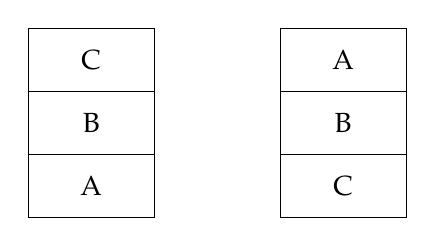
\begin{tikzpicture}[scale=0.8]
  % Initial configuration
  \draw (0,0) rectangle (2,1) node[midway] {A};
  \draw (0,1) rectangle (2,2) node[midway] {B};
  \draw (0,2) rectangle (2,3) node[midway] {C};

  % Goal configuration
  \draw (4,0) rectangle (6,1) node[midway] {C};
  \draw (4,1) rectangle (6,2) node[midway] {B};
  \draw (4,2) rectangle (6,3) node[midway] {A};
\end{tikzpicture}
\label{fig:intro-blocks}
\end{figure}

Planning tasks are solved by planners, which are software systems designed to find plans for given planning problems. Planners employ various algorithms and techniques to explore the search space of possible operators and states in order to find an optimal or satisfactory plan. Planners typically take as input a formal representation of the planning problem, including the initial state, goal condition, and a set of available operators. The formal representation of a planning task can be specified using various notations.

\section{Heuristic Search}
To solve planning tasks, planners commonly use a best-first search algorithm, which uses a function~$f$ to guide the search. The function $f$ combines the current cost $g(s)$ of a partial sequence of operations initiated from the initial state and reaching state $s$, along with a heuristic function $h(s)$ that provides an estimate of the cost-to-goal (also known as heuristic value or $h$-value) from state $s$. For example, \astar search is guided by $f(s)=g(s)+h(s)$~\cite{hart-et-al-ieeessc1968}, and greedy best-first search (\gbfs) is guided only by $f(s)=h(s)$~\cite{doran-michie-rsl1966}. In general, best-first search algorithms prove more effective when the heuristic function~$h$ better approximates the optimal heuristic function~\hstar.

%In particular, GBFS organizes states in a priority queue ordered by their cost-to-goal estimate, which is provided by the heuristic function. By expanding states with the lowest cost-to-goal estimate, GBFS finds a solution.
Various domain-independent heuristics efficiently calculate the cost-to-goal estimate of a state using domain logic, which includes specific information that aids in reasoning about operators and rules, such as mutexes indicating impossible states. Examples include delete relaxation~\cite{Hoffmann.Nebel/2001}, landmarks~\cite{hoffmann-et-al-jair2004,Karpas.Domshlak/2009}, critical paths~\cite{haslum-geffner-aips2000}, and state equation~\cite{bonet-ijcai2013}.

\section{Preferred Operators}
Preferred operators are used in conjunction with heuristic functions and can aid planners in reducing the number of expanded states during a search process~\cite{Helmert/2006,Richter.Helmert/2009}. Intuitively, preferred operators generate successor states that are closer to the goal. By prioritizing the expansion of states generated by preferred operators, planners benefit from additional guidance, often resulting in a higher success rate for solving tasks compared to only relying on the heuristic function. Learning preferred operators shares similarities with learning policies, as both involve the selection of actions that are more likely to result in desirable outcomes. The existing methods for identifying preferred operators are currently limited to symbolic-based (also called as logic-based) approaches. The most effective approach used at present involves using the preferred operators calculated alongside the Fast-Forward (FF) heuristic~\cite{Hoffmann.Nebel/2001}, as implemented in the Fast Downward planning system~\cite{Helmert/2006}. Preferred operators are particularly beneficial in competitive scenarios, as they maximize the number of solved tasks (coverage). Planners incorporating preferred operators emerged as winners in the satisficing track of the International Planning Competition (IPC) in 2004, 2008, 2011, and 2018~\cite{Helmert/2006,Richter.lama.etal/2011,Richter.lama.etal/2011,Seipp-fast.etal/2018}.

\section{Deep Learning}
Deep learning, as described by~\citet{Goodfellow.etal/2016}, is a subfield of machine learning that focuses on the design and training of neural networks (NNs) with multiple layers. It revolves around the concept of learning hierarchical representations of data, where each layer in the network progressively extracts more complex and abstract features. Through the use of deep neural networks, deep learning algorithms can automatically discover and capture intricate patterns from large-scale datasets in a varity of tasks, including image classification, speech recognition, natural language processing, and more.

Deep learning models can learn in different ways. This study focuses on supervised learning, which involves using labeled datasets to classify or make predictions. In this case, a dataset used to train an NN can be represented as multiple pairs in the format $(y, x)$. Here, the target $y$ refers to the desired output or label associated with a specific input instance $x$. Deep learning models can effectively learn and generalize from the provided labeled data to make accurate predictions or classify new, unseen inputs.

\section{Learning in Planning}
In recent years, interest in using NNs to learn heuristic functions~\cite{Ferber.etal/2020a,Yu.etal/2020,Shen.etal/2020,Ferber.etal/2022,OToole/2022} or policies~\cite{Toyer.etal/2018,Toyer.etal/2020,Stahlberg.etal/2022} to solve planning tasks has increased. For supervised methods, the general approach is to generate a set of samples as pairs of states and cost-to-goal values and use them to train a neural network. However, it is challenging to learn effective heuristic functions, since (a) state spaces tend to grow exponentially in size as the amount of information needed to describe them increases, but the portion of the state space that we can actually sample is relatively small, (b) symbolic-based heuristics can be applied to any domain, while learned heuristics are hard to transfer, and (c) learned heuristics are generally slow to compute, thus they need to be for informed, i.e., expand fewer states when compared to symbolic-based heuristics to reach the goal. These challenges also apply to learning preferred operators.

\section{Contributions}
This study represents the first attempt to discover preferred operators from a sample set and use an NN to learn them. We present a new sampling method and a novel sample-based technique for identifying preferred operators. The technique involves backward search from the goal (also known as regression), constructing a graph with sampled states representing their successor-predecessor relationships, and determining for each state the set of operators used to reach the goal as preferred operators. This study reveals that a neural network can learn the preferred operators from a subset of the state space and effectively extend this learning to the entire state space across diverse planning domains. The proposed approach outperforms the current best symbolic-based preferred operator method in the benchmark tasks. In particular, this work presents:

\begin{itemize}
\item A systematic study of preferred operators.
\item A new sampling method tailored for discovering preferred operators.
\item A novel method based on shortest path graphs to discover preferred operators in an existing sample set.
\item An analysis of the quality of the learned preferred operators and a comparison to existing symbolic-based methods.
\end{itemize}
%
% - - - - - - - - - - - - - - - -- - - - - -
% background
% - - - - - - - - - - - - - - - -- - - - - -
% these are all things that exist already
% and that the reader needs to know before
%
\chapter{Background}
This chapter serves as a foundation, providing essential information for comprehending the subsequent chapters of this work. In particular, we present the notation employed in this work along with the essential concepts required for a comprehensive understanding of the subject matter.

\section{Classical Planning Notation}
In this section we present three ways to represent a classical planning task. The first one, STRIPS~\cite{Fikes.Nilsson/1971}, represents a planning task using propositional facts (Boolean variables). The second way, \sas~\cite{Backstrom.Nebel/1995}, represents a planning task using multi-valued state variables. The third way, PDDL~\cite{Ghallab.etal/1998}, is based on predicate logic and is commonly used for writing planning tasks to be used as input for planners.

\subsection{STRIPS}
% A planning task in STRIPS is defined as $\Pi = \langle F, O, I, G\rangle$ where $F$ is a set of facts (Boolean variables), $O$ is a set of operators or actions over $F$, where $\langle Pre(o), Add(o), Del(o) \rangle \subseteq F$, $I \subseteq F$ is the initial state, and $G \subseteq F$ is a a set of goal facts that must be satisfied. We say that operators $O(s)$ are \emph{applicable} in $s$ if they satisfy $Pre(o)$. We progress a state $s$ with operator $o$ by setting the propositions in $Add(o)$ to true and $Del(o)$ to false. Finally, a sequence of operators $\pi=(o_1,\ldots,o_k)$ applicable to the initial state is called a plan.
A planning task in STRIPS representation is defined by~$\Pi=\langle\mathcal{P},\mathcal{O},\mathcal{I},\mathcal{G}\rangle$. Here, $\mathcal{P}$~is a set of propositions, $\mathcal{O}$~is a set of operators, $\mathcal{I} \subseteq \mathcal{P}$~is an initial state, and $\mathcal{G}$~is a set of goal states. Each assignment $s \subseteq \mathcal{P}$ represents a state, and the set~$\mathcal{S}$ of all states over $\mathcal{P}$ is the state space.
An operator~$o \in \mathcal{O}$ is defined by a triple~$\langle\pre(o),\add(o),\del(o)\rangle$ that specifies its preconditions, add-effects and delete-effects, respectively. We say that operator $o$ is applicable to state $s$ if its preconditions are satisfied by $s$, i.e., $\pre(o) \subseteq s$, and it produces a successor state~$s' = \sucs(s,o) = (s \setminus \del(o)) \cup \eff(o)$. In other words, we progress a state $s$ with operator $o$ by setting the propositions in $add(o)$ to true and in $del(o)$ to false. The set of successor states of $s$ is denoted by~$\sucs(s)=\{\sucs(s,o)\mid o\in \mathcal{O}, \pre(o) \subseteq s\}$.
A sequence of operators~$\pi=o_1,\ldots,o_k$ is valid for a state~$s_0$ if produces a sequence of states~$s_1,\ldots,s_k$ for $s_i=\sucs(s_{i-1},o_i)$. A sequence~$\pi$ for the initial state~$\mathcal{I}$ is called a plan if $s_k \in \mathcal{G}$, and its cost is given by $|\pi| = k$ since we are considering only unitary costs. The plan with minimum length is an optimal plan.

Heuristics based on delete-relaxation obtain the heuristic from a \emph{relaxed} version of the planning task. A relaxed planning task in STRIPS is defined as $\Pi^{+}=\langle\mathcal{P},\mathcal{O'},\mathcal{I},\mathcal{G}\rangle$, where $\mathcal{O'} = \{ \langle \pre(o), \add(o), \emptyset \rangle \,|\, o \in O \}$, i.e., the delete-effects of the planning task are ignored. Relaxed tasks can be solved efficiently even though finding the optimal solution is $\mathcal{NP}$-hard~\cite{Bylander/1994}. For example, the heuristic \hadd approximates the optimal heuristic value for a state $s$ as the sum of the costs of achieving each proposition in $G$ independently of the others.

\subsection{\sas}
In this study, we use the \sas representation to describe classical planning tasks independent of any particular domain. A \sas planning task is defined as $\Pi=\langle\mathcal{V},\mathcal{O},s_0,s^*\rangle$, where $\mathcal{V}$ is a set of state variables, and each variable $v\in \mathcal{V}$ has a finite domain~$\dom(v)$, that represents a set of mutually exclusive propositions called mutexes (variables from different domains can also be mutexes), $\mathcal{O}$ is a set of operators where each operator $o \in \mathcal{O}$ is defined as a pair of preconditions and effects $(\pre(o),\eff(o))$, both partial states~$s$ defined as a partial function $s:\mathcal{V}\rightarrow \mathcal{D}$, where $\mathcal{D}=\cup_{v\in \mathcal{V}}\dom(v)$, such that $s(v)\in \dom(v)$ whenever $s(v)$ is defined, otherwise, $s(v)$ is undefined and written as $s(v)=\bot$.  A (complete) state $s$ is a partial state defined on all variables in~$\mathcal{V}$. The state~$s_0$ defines the initial state, and the partial state~$s^*$ defines the goal condition, where $s_0, s^* \in \mathcal{S}$ and $\mathcal{S}$ is the set of all states (or state space).
%the expression $\mathcal{D}=\cup_{v\in \mathcal{V}}\dom(v)$ means that the domain of $\mathcal{D}$ is the union of the domains of all the elements in $\mathcal{V}$. That is, the set of values that $\mathcal{D}$ can take is the combination of all the values that each element in $\mathcal{V}$ can take.
An operator $o \in \mathcal{O}$ is applicable to a state $s$ if its preconditions are fulfilled by $s$, denoted by $\pre(o) \subseteq s$, and it generates a successor state $s'=\sucs(s,o):=\eff(o)\circ s$. Here, $s'=t\circ s$ is defined as $s'(v)=t(v)$ for all $v$ such that $t(v)$ is defined, and for all other cases, $s'(v)=s(v)$. The set of all successor states resulting from state $s$ is denoted by $\sucs(s)=\{{\sucs(s,o)\mid o\in \mathcal{O}, \pre(o) \subseteq s}\}$. A sequence of operators $\pi=(o_1,\ldots,o_k)$, where $o_i\in \mathcal{O}$, is considered valid for the initial state $s_0$ if, for $i\in[k]$, operator $o_i$ can be applied to $s_{i-1}$, and it produces $s_i=\sucs(s_{i-1},o_i)$. A plan refers to a valid sequence $\pi$ for $s_0$ such that $s^* \subseteq s_k$. In this work, all operators have unit costs, so the plan length is $|\pi| = k$.

The predecessor of a partial state $s$ under operator $o$, denoted $\pred(s,o)$, can be obtained through a process called regression. Regression involves determining the predecessor state that can lead to the current partial state by applying the operator $o$. An operator $o$ is considered relevant for partial state $s$ if at least one defined effect in $o$ is applicable to $s$, and consistent if the operator agrees with the defined effects in $s$. An operator $o$ is said to be \emph{backward applicable} in partial state $s$ if it is both relevant and consistent with $s$, and it leads to a predecessor $r$ given by $r=\pre(o)\circ (s|_{\dom(s)\setminus\eff_r})$. Note that $\sucs(r,o)\subseteq s$ may differ from $s$.
A partial state $s$ has predecessors $\pred(s)=\{{\pred(s,o)\mid o\in \mathcal{O}}\}$ where $o$ is backward applicable to $s$, and a regression sequence from state $s_0$ is valid if $o_i$ can be applied to $s_{i-1}$ and produces $s_i=\pred(s_{i-1},o_i)$. All partial states~$s_k$ can reach a partial state $s\subseteq s_0$ in at most $k$ forward applications of the reversed operator sequence.
If a valid regression sequence $\rho=(o_1,\ldots,o_k)$ is generated, a sequence of partial states that can reach the goal in at most $k$ steps will be produced since the goal is a partial state.

The backward state space (BSS) refers to the set of partial states that can be reached from the goal state $s^*$ by applying backward applicable operators. The BSS is explored during regression. Conversely, the forward state space (FSS) pertains to the set of states that can be reached from the initial state $s_0$ by applying a sequence of operators. The FSS is explored when solving a task.

\subsection{PDDL}
We can also represent a classical planning task using PDDL. Tasks specified in PDDL are written in a Lisp-like syntax and are separated into two definitions, the domain, which specifies the actions and predicates, and the problem, which specifies the objects, the initial state, and the goal condition.

For example, in Blocks World, $(ontable~?x)$ represents a predicate that indicates if a block $x$ is on the table or not, and $(pickup~?x)$ is an action that defines the act of picking up block $x$. This action is further specified by a set of preconditions $(and~(clear~?x)~(ontable~?x)~(handempty))$ that must hold true before $(pickup~?x)$ is applied, i.e., $x$ must be clear (no other block above it), $x$ must be on the table, and the hand must be empty. The effects of applying $(pickup~?x)$ are $$(and~(not~(ontable~?x))~(not~(clear~?x))~(not~(handempty))~(holding~?x)),$$

that is, $x$ is not on the table, $x$ is not clear, the hand is not empty, and the hand is holding $x$.

\section{Heuristic Functions}
A heuristic function $h:\mathcal{S}\rightarrow \mathbb{R}^{\geq 0}\cup\{\infty\}$ estimates the optimal plan length from a state $s$ to the goal $s^*$, where the optimal heuristic function is defined as $\hstar(s) = |\pi_{s}^{*}|$, i.e., the length of the true plan from $s$ to $s^{*}$. Heuristic functions are used to guide search algorithms, optimization techniques, or decision-making processes by providing informed estimates or approximations based on available information or problem-specific knowledge. The goal of a heuristic function is to efficiently guide the search or decision-making process towards more promising paths or solutions, even in the absence of complete or perfect information. A heuristic function can have several properties that indicate its quality, such as:

\begin{itemize}
        \item Admissibility: $h(s) \le \hstar{(s)}$, i.e., the heuristic never overestimates the true cost-to-goal.
        \item Consistency (or monotonicity): $h(s) + cost(o) \ge h(s')$ for all $s \xrightarrow{o} s'$.
        \item Goal-awareness: $h(s) = 0$ for all goal states.
        \item Safeness: all states have $h(s) = \infty$ if $\hstar (s) = \infty$, for example in dead-ends.
\end{itemize}

Heuristics are typically derived from a model of the task, such as the \sas model introduced earlier, but can also be obtained by learning the map of some state $s$ to its heuristic value $h(s)$, where the desired output of the NN can be either the direct cost-to-goal estimates or some form of encoding representing these estimates.

A propositional representation of a state is better suited for learning heuristic functions over states. For this purpose, consider a planning task denoted as $\Pi=\langle\mathcal{V},\mathcal{O},s_0,s^*\rangle$. Here, $\mathcal{V}=\{v_1,\ldots,v_n\}$ represents a set of variables, and $D(v_i)=\{d_{i1},\ldots,d_{i,s_i}\}$ represents the domains of variable $v_i$, with $i\in[n]$. To represent any state $s$, we use a sequence of facts denoted as
% The domain consists of possible values that $v_i$ can take. The values are represented as $d_{i1}$ to $d_{i,s_i}$, where $s_i$ indicates the number of possible values for $v_i$.
$$\mathcal{F}(s)=(f_{11},f_{12},\ldots,f_{1,s_1},\ldots,f_{n1},f_{n2},\ldots,f_{n,s_n}),$$ where each fact $f_{ij}=[s(v_i)=d_{ij}]$ indicates whether variable $v_i$ assumes the value $d_{ij}$ in state $s$. It is important to note that the facts $\mathcal{F}_i=\{f_{i1},\ldots,f_{i,s_i}\}$ corresponding to variable $v_i$ adhere to the consistency condition $\sum_{f\in \mathcal{F}_i} f\leq 1$, as each variable can take at most one value, and $\sum_{f\in \mathcal{F}_i} f=0$ only when $v_i$ is undefined. In a more general sense, given a set of propositions $\mathcal{P}$, we express $\mutex(\mathcal{P})$ when the constraint $\sum_{p\in \mathcal{P}} [p]\leq 1$ must be satisfied within the states of $\Pi$. Planning systems can typically deduce mutexes from the description of the planning task $\Pi$~\cite{Helmert/2009}.

\section{Greedy Best-First Search}
Greedy Best-First Search (GBFS, \cref{alg:gbfs}) is a best-first search algorithm typically employed by planners to solve planning tasks by exploring the FSS. The GBFS algorithm organizes states in a priority queue based on their cost-to-goal estimate, which is determined by the heuristic function. GBFS explores states with the \emph{lowest} cost-to-goal estimate first in order to find a solution. Since GBFS typically only considers the cost-to-goal estimate of a state to guide the search, it is commonly used to verify the quality of a heuristic function.

\begin{algorithm}
\caption{Greedy Best-First Search (GBFS)}
\label{alg:gbfs}
\begin{algorithmic}[1]
\Procedure{GBFS}{$\Pi, \text{heuristic}$}
  \State Initialize an empty priority queue $pqueue$
  \State Mark the initial state $s_0$ as visited
  \State Insert $s_0$ into $pqueue$ with priority $\text{heuristic}(s_0)$

  \While{$pqueue$ is not empty}
    \State $s \gets$ state with the highest priority in $pqueue$

    \If{$s$ satisfies the goal state $s^{*}$}
      \State \textbf{return} the solution
    \EndIf

    \ForAll{successor states $s'$ of $s$}
      \If{$s'$ has not been visited}
        \State Mark $s'$ as visited
        \State Insert $s'$ into $pqueue$ with priority $\text{heuristic}(s')$
      \EndIf
    \EndFor
  \EndWhile

  \State \textbf{return} failure (no solution found)
\EndProcedure
\end{algorithmic}
\end{algorithm}

\section{Preferred Operators}
\label{sec:background-preferred-operators}
Preferred operators can be described as operators that, given a particular state $s$, tend to generate successors that are more likely to lead to the goal state when compared to other successors of $s$. Preferred operators provide a way to prioritize the expansion of certain states over others during the search. Although the method of identifying preferred operators depend on implementation, the first approach was introduced in the original Fast-Forward (FF) planner~\cite{Hoffmann.Nebel/2001}, where preferred operators are calculated alongside the FF heuristic. Specifically, the FF planner returns a relaxed Graphplan~\cite{Blum.etal/1997} from the relaxed task, and the cost-to-goal estimate for a state $s$ is defined as the length of the plan obtained for $s$, while the preferred operators for state $s$ are the operators of the plan applicable in $s$. The Graphplan algorithm is a planning algorithm that operates on a graph representation of a planning problem. It constructs a layered planning graph by expanding a state and applying actions to generate subsequent layers. It checks if the goal state is reachable and, if so, extracts a valid plan from the graph.

The current approach to extract preferred operators is the one implemented in the Fast Downward planning system~\cite{Helmert/2009}, based on so-called domain transition graphs (DTGs), compatible with multi-valued variables, where the preferred operators obtained with the calculation of the FF heuristic are the current best. The DTG provides a compact representation of the state space by capturing the dependencies between variables and their possible values, where each variable in the planning domain is represented as a node, and the transitions between different values of the variable are represented as edges between the nodes. The DTG for variable $v$ has a transition $d \xrightarrow{o} d'$ if there exists an operator that can modify the value of $v$ from $d$ to $d'$.

To support preferred operators, Fast Downward extends the textbook implementation of GBFS (\cref{alg:gbfs}) to use a dual-queue approach. In this setup, there are two queues: the ``default queue'' receives all generated states (representing the default behavior without preferred operators), and the ``preferred queue'' only accepts states generated by preferred operators. States are expanded from both queues in an alternating manner or may use \emph{boosting}~\cite{Richter.Helmert/2009}. With a boost value $n$, if the search expands a state with an $h$-value lower than all previously expanded states (indicating progress in the search), the preferred queue is used for the subsequent $n$ expansions, as long as it contains elements. Furthermore, the boost value is cumulative, meaning that whenever the search progresses, $n$ expansions are added to the remaining number of subsequent expansions from the preferred queue.

\section{Neural Networks}
A standard NN architecture is composed of an input layer, one or more hidden layers, and an output layer. Each neuron in the hidden layers applies a nonlinear transformation to a weighted sum of the inputs it receives. The weights and biases of the neurons are learned through a process called backpropagation, which optimizes a loss function using gradient descent or its variants. For details on backpropagation and gradient descent, refer to~\citet{Goodfellow.etal/2016}.\ppi{Do I need to explain backpropagation and gradient descent in detail?}

The mean squared error (MSE) loss function is commonly used for regression problems, where the goal is to predict continuous values. Given a prediction $\hat{y}$ and the corresponding target value $y$, the MSE loss is calculated as the mean of the squared differences between the prediction and the target:

$$\text{MSE}(\hat{y}, y) = \frac{1}{N} \sum_{i=1}^{N} (\hat{y}_i - y_i)^2,$$

where $\hat{y}_i$ represents the $i$-th element of the prediction vector $\hat{y}$, $y_i$ represents the $i$-th element of the target vector $y$, and $N$ is the total number of elements in the vectors.

The binary cross-entropy (BCE) loss function is commonly used for binary classification problems, where the goal is to predict a binary outcome, or multi-label classification problems where there can be more than one correct outcome~\cite{Tsoumakas.etal/2007}.
Given a prediction $\hat{y}$ and the corresponding binary target value $y$, the BCE loss is calculated as the average of the element-wise cross-entropy between the prediction and the target:

$$\text{BCE}(\hat{y}, y) = -\frac{1}{N} \sum_{i=1}^{N} \left[y_i \log(\hat{y}_i) + (1 - y_i) \log(1 - \hat{y}_i)\right],$$

where $\hat{y}_i$ represents the $i$-th element of the prediction vector $\hat{y}$, $y_i$ represents the $i$-th element of the target vector $y$, and $N$ is the total number of elements in the vectors.

This study implements a feedforward neural network with residual blocks. Let us consider a feedforward neural network with L layers. For simplicity, we assume each layer has the same number of neurons, denoted by N. The input to the network is represented $x$, and the output is denoted by $y$. The activation function of a neuron in the $l$-th layer is denoted as $a^l(\cdot)$, and the weights connecting the $i$-th neuron in layer $l-1$ to the $j$-th neuron in layer $l$ are denoted as $w^{l}_{ij}$. The bias of the $j$-th neuron in layer $l$ is denoted as $b^{l}_{j}$. The output of the $j$-th neuron in layer $l$ is given by:

$$z^{l}_{j} = \sum_{i=1}^{N} w^{l}_{ij} a^{l-1}_{i} + b^{l}_{j}$$

The activation of the $j$-th neuron in layer $l$ is then computed as:

$$a^{l}_{j} = a^{l}(z^{l}_{j})$$

Common activation functions include sigmoid, rectified linear units (ReLU), and tanh~(\cref{fig:activation-functions}).

\begin{figure}[ht]
%\captionsetup{skip=5pt}
\caption{Sigmoid, ReLU, and tanh activation functions.}
%\centering
\centerline{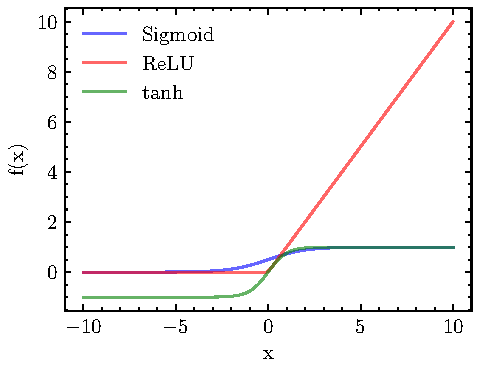
\includegraphics[]{img/sigmoid-relu-tanh}}
\label{fig:activation-functions}
\end{figure}

Standard NNs may suffer from the vanishing gradient problem~\cite{Bengio.etal/1994}. The gradients tend to diminish as they propagate backward through multiple layers, making it challenging for earlier layers to learn meaningful representations. This issue hampers the optimization process and limits the network's overall performance.

To address this challenge, Residual Neural Networks (ResNets)~\cite{He.etal/2016} were introduced. ResNets use skip connections or shortcuts that bypass one or more layers, allowing the information to flow directly from one layer to another. This bypassing mechanism mitigates the vanishing gradient problem and facilitates the training of very deep networks. Let us consider a ResNet architecture with L layers. The output of the $l$-th layer is denoted by $a^{l}$, and the output of the previous layer is denoted by $a^{l-1}$. The residual connection between the $l$-th and $l-1$-th layers can be represented as:

$$a^{l} = a^{l-1} + \mathcal{F}(a^{l-1}, W^{l}),$$

where $\mathcal{F}$ represents a residual function, typically implemented as a convolutional or fully connected layer, and $W^{l}$ denotes the learnable parameters of this function.


\chapter{Related Work}
In this chapter, we review and discuss the previous research conducted on topics related to the subject matter of this study.

\section{Obtaining Preferred Operators}
The first notion of preferred operators as currently used were described by~\citet{Hoffmann.Nebel/2001} and implemented in the FF planner, then called \emph{helpful actions}. The current most effective approach for identifying preferred operators uses the computation of the FF heuristic as implemented in the Fast Downward planning system~\cite{Helmert/2006}.
Furthermore, \citet{Richter.Helmert/2009} performed a systematic study on how best to use preferred operators and showed that the dual-queue approach described in~\cref{sec:background-preferred-operators} yielded the best results.

\section{Learning Heuristic Functions}
While prior research has not specifically addressed learning preferred operators, there have been numerous studies on using learning heuristic functions for classical planning. These studies can be categorized into two primary approaches.
The first approach heavily relies on domain logic to generate samples and instantiate networks. Its objective is to generalize across domains or a planning formalism.
On the other hand, the second approach minimally employs domain logic solely for generating samples and focuses on generalization within a state space.

The first approach uses ``structured'' neural networks with architectures specifically designed to align with the characteristics and requirements of the given input task. Examples include learning domain-independent heuristic functions with hypergraph neural networks~\cite{Shen.etal/2020}, and learning policies with action schema networks~\cite{Toyer.etal/2018,Toyer.etal/2020} and graph neural networks~\cite{Stahlberg.etal/2022}. These approaches offer higher expressive power and can be applied regardless of the state spaces. However, they heavily rely on domain logic. Furthermore, the major limitation of this set of approaches is that they can not be used to solve planning tasks of the size typically solved by planners as they require excessive memory for instantiation or are too slow in expanding the necessary number of states.

This work follows the second approach, employing supervised learning to train a feedforward neural network with pairs of states and cost-to-goal estimates~\cite{Ferber.etal/2020a,Yu.etal/2020,Ferber.etal/2022,OToole/2022}. Samples can be generated with forward search from the initial state~\cite{Ferber.etal/2020a}, backward search from the goal~\cite{Yu.etal/2020,OToole/2022}, or a combination of both~\cite{Ferber.etal/2022}.

In this context,~\citet{Ferber.etal/2020a} conducted a systematic study on the hyperparameters of the feedforward neural network architecture and found that their influence is secondary. They discovered that, for a fixed architecture, two main factors significantly impact the informativeness of the heuristic: the selection of the sample subset and the size of the sample set.

Furthermore,~\citet{Yu.etal/2020} and~\citet{OToole/2022} performed backward searches from the goal state.~\citet{Yu.etal/2020} employed depth-first search, while ~\citet{OToole/2022} used random walks. In both cases, the cost-to-goal estimates were assigned as the lowest depth at which the states were generated.~\citet{Ferber.etal/2022} used a combination of backward and forward searches. To concurrently generate samples and learn a heuristic function,~\citet{Ferber.etal/2022} employed a bootstrapping method~\cite{Arfaee.etal/2011}, where initially new initial states are generated using backward random walks, which are then solved using GBFS guided by the learned heuristic. The resulting plans yield samples, with each sample corresponding to a state within the plan and its associated cost-to-goal estimate. These samples are subsequently used to further train the neural network, aiming to enhance the learned heuristic.
% O'Toole (2022) also presented a method for generating samples that does not involve expansions. This method includes randomly generating states with high cost-to-goal estimates and including them in the sample set. O'Toole demonstrated that this approach substantially increases coverage.

This second set of approaches offers the advantage of requiring minimal computational resources. However, a limitation is that the trained models are typically applicable only within the specific state space they were trained on. These approaches rely on domain logic to a lesser extent, and only during sample generation, such as determining applicable operators and mutexes. Moreover, in cases where a black-box simulator is accessible to generate predecessor and successor states, which can also be learned, these approaches can eliminate the requirement for domain-specific logic entirely.


%
% - - - - - - - - - - - - - - - -- - - - - -
% sample generation
% - - - - - - - - - - - - - - - -- - - - - -
% now we talk about the stuff we're doing
%
\chapter{Sample Generation}
\label{cha:sample-gen}
This chapter presents the methods we use to generate samples for training, specifically to train a neural network that predicts $h$-values (\cref{sec:sample-learn-h}), and another to train a neural network that identifies preferred operators (\cref{sec:sample-learn-po}).

There are multiple techniques available to generate a sample set for training neural networks in planning. These techniques include search methods like breadth-first search (BFS), depth-first search (DFS), and random walk (RW). In search methods, the generation of the sample set typically begins from a source node, which is commonly the initial state for forward search or the goal state for backward search (regression). Random sampling of the state space can also be employed to generate the sample set. Unlike search methods, random sampling produces independent samples, as each state is generated without relying on previous samples. The distribution of samples across the state space can impact the generalization performance of the neural network. This impact can vary depending on the specific sampling algorithm used.

\section{Sampling for Learning Heuristic Functions}
\label{sec:sample-learn-h}
To learn heuristic functions, states are labeled with a cost-to-goal estimate during sampling. In regression-based methods, the value assigned to a sampled state is determined by its distance to the goal. To generate samples, we use regression to expand the backward state space. Specifically, we use a combination of BFS with RW, named \bfsrw.

A regression rollout refers to a sequence of state expansions, which concludes under two conditions: either when the last expanded state has no predecessors or when it reaches the depth limit $L$. The process of generating samples halts once the desired number of samples $N$ has been attained. Random walks can have multiple rollouts due to the depth limit $L$, whereas BFS has a single rollout. However, if the backward state space contains an insufficient number of states to generate the required $N$ samples, BFS may need to perform multiple rollouts.

Different expansion strategies generate sample sets with varying distributions of optimal distances from the goal. To address this, we propose a novel approach called \bfsrw, combining BFS and random walks. \bfsrw aims to achieve good coverage near the goal while obtaining a diverse set of samples from the remaining state space.

\bfsrw consists of two phases. In the first phase, a fixed percentage $p_\bfsrw$ of the $N$ samples is generated using BFS. The BFS expands a state from layer $k$ and generates $n$ states from layer $k+1$. These states are sampled only if the total samples plus $n$ are within $p_{\bfsrw}N$; otherwise, no states are sampled, and BFS expands another state. The set of unexpanded samples, i.e., leaves, is denoted as $Q$. The second phase involves multiple random walk rollouts starting from states in $Q$, selected randomly with replacement after all states have been chosen once. This process continues until the sample set reaches $N$. During the random walk phase, states sampled in the BFS phase are discarded.

\ppi{Add pseudocode.}

\subsection{Maximum Regression Limit}

In previous work by \citet{Yu.etal/2020} and \citet{OToole/2022}, a maximum limit $L$ of $200$ and $500$, respectively, has been used to restrict expansion depth. However, using a fixed limit may not be the optimal choice for tasks with state spaces of varying diameters or different maximum distances to a fixed goal when seeking a representative sample of the state space. This becomes particularly problematic in regression, as an overestimated maximum regression limit $L$ can result in inflated cost-to-goal estimates, while an underestimated limit can lead to an excessive concentration of samples near the goal.

Hence, it is essential to determine the optimal maximum regression limit for a fixed goal as a function of the longest distance \distfarthest between the goal state and any potential initial state. While BFS can provide an accurate estimate of \distfarthest, DFS and random walks need higher limits due to their tendency to deviate from the shortest paths. Since the exact value of \distfarthest is typically unknown, we propose an adaptive and approximated approach to define the maximum regression limit $L$ based on the input task parameters. This adaptive method allows us to tailor the limit according to the specific characteristics of the task.
Thus, we set the regression limit to $L=\bar F=\ceil{\facts/\overline{\eff}}$ where $\overline{\eff}=\sum_{o\in \mathcal{O}} |\eff(o)|/|\mathcal{O}|$, i.e.,~the number of facts per mean number of effects in the operators.

\subsection{Sample Completion}
Regression sampling generates a set of partial states with undefined variables. However, during the search, the NN is trained on and expects complete states as input.
Each partial state can be completed by assigning a value $s(v)\in\dom(v)$ to all fact pairs $(v,s(v))$ where $s(v)=\bot$.
To complete partial states, we employ a method that assigns a random value $s(v) \in \dom(v)$ to each undefined variable. However, we ensure that the assigned values satisfy mutexes derived from the planning task. We process the undefined variables in a random order and assign them random values that do not violate the mutexes. If, after $10$\,K attempts, we are unable to complete the state, we leave the corresponding facts undefined, setting them to false (zero)\footnote{In practice, this situation is extremely rare, occurring in only about $0.1\,\%$ of the samples.}.

\subsection{Randomly Generated Samples}
\citet{OToole/2022} demonstrated that augmenting a sample set generated through expansion with randomly generated samples enhances the performance of the search algorithm guided by the learned heuristic. They suggest assigning a cost-to-goal estimate of $L+1$ to randomly generated samples, where $L$ represents the maximum regression limit.
The samples are generated from undefined states and are completed as discussed earlier. If the generated state $s$ is already present in the sample set, denoted as $s = s_i$ for some $i\in[N]$, it is assigned the cost-to-goal estimate $h_i$. Conversely, if the state $s$ is not already in the sample set, it is given a cost-to-goal estimate of $1+\max_{i\in[N]} h_i$, ensuring that the estimate is larger than all existing estimates.

\subsection{Improving Cost-to-Goal Estimates}

Let us begin by noting that cost-to-goal estimates always provide a lower bound on the true cost-to-goal $h^{*}$, as explained below.

\begin{property}
\label{prop:hvalue}
The cost-to-goal estimate $h(s)$ of a sample $s$ obtained by regression satisfies $h(s)\geq h^*(s)$.
\end{property}

\begin{proof}
This follows because each estimate is witnessed by a plan.
A valid regression sequence $\rho=(o_1,\ldots,o_k)$ produces a series of partial states that can reach the goal within a maximum of $k$ steps and with a cost no greater than $\sum_{i\in[k]}\text{cost}(o_i)$. The cost of this sequence cannot be lower than the optimal cost.
\end{proof}

Better $h$-value estimates generally result in improved learned heuristics, leading to fewer expanded states during a search. However, this correlation is not always guaranteed~\cite{Holte/2010}. To enhance the cost-to-goal estimates while preserving \cref{prop:hvalue}, we employ two straightforward techniques. The first method, called \sai, minimizes estimates across repeated samples, while the second method, known as \sui, minimizes estimates across the successors of samples.


\subsubsection{Sample Improvement}
It is possible to generate duplicate states with different estimates due to multiple random walk rollouts. To address this, we update the cost-to-goal estimate for each sampled state $s$ to the minimum estimate $h(s) = \min\{h_i \mid s=s_i, i\in[N]\}$. This update is applied to both partial and complete states since identical complete states can be generated from different partial states. We refer to this procedure as ``sample improvement'' (\sai). Choosing the minimum $h$-value is sound because valid plans from a regression witness these distances. Consequently, \cref{prop:hvalue} remains valid.

\subsubsection{Successor Improvement}
In addition to sampling the same states, it is common to sample neighboring states in the state space, especially for states close to the goal. We can leverage this to enhance the cost-to-goal estimates using the following approach. Let $G=(V,A)$ be a directed graph representing all sampled partial states, where~$V=\{s_i\mid i\in[N]\}$. For every pair of states $s$ and $t$ in $V$, if there exists an operator $o\in\mathcal{O}$ applicable to $s$ such that $\sucs(s,o)\subseteq t$, we add an arc $(s,t)$ of length $\text{cost}(o)$ to $A$. Note that, unlike in regression, if $\pre(o)$ mentions to an undefined variable in $s$, then $o$ is not applicable. To efficiently handle subsets, we store all samples in a trie and search for successors in states that are supersets. For partial states generated by regression, there is always at least one successor, except for the goal state $s^*$. We then compute the shortest paths to the goal in the graph $G$, for example, using the Dijkstra algorithm, and update the cost-to-goal estimates accordingly. We refer to this procedure as ``successor improvement'' (\sui). Since all distances are supported by plans, \cref{prop:hvalue} is preserved.

\section{Sampling for Learning Preferred Operators}
\label{sec:sample-learn-po}
The sample generation approach described in~\cref{sec:sample-learn-h} is not suitable for learning preferred operators due to the presence of duplicate samples within rollouts. This leads to a sample set that contains numerous repeated samples, which offer no additional value when constructing the shortest path graph for identifying preferred operators. Consequently, this approach fails to effectively explore the state space and identify additional preferred operators. To address this limitation, we have developed an alternative sample generation method specifically designed to discover preferred operators, divided into two phases.

Let $S_1$ and $S_2$ denote the sets of samples generated in the first and second phases, respectively. The complete sample set is represented by $S = S_1 \cup S_2$, consisting of $N$ samples, where $S = \{ s_1, s_2, \ldots, s_n\}$ with distinct elements $s_i \neq s_j$ for $i \neq j$. Let $k_1$ and $k_2$ be variables satisfying $k_2 = 1 - k_1$ if $k_1 > k_2$, and $k_1 = 1 - k_2$ if $k_1 < k_2$, where $0 < k_1 < 1$ and $0 < k_2 < 1$.
In the first phase, we use BFS by applying backward applicable operators from the goal state until expanding $k_1N$ states, which are then added to $S_1$.
In the second phase, we maintain an open queue, containing states generated but not yet expanded, and a closed queue, comprising states that have been expanded and already sampled. During each iteration, we randomly select a state from the open queue, move it to the closed queue, add it to the sample set $S_2$, and insert its predecessors into the open queue if they are not already present in either queue. The sampling process continues until $|S_2| = k_2N$.

\ppi{Add pseudocode.}

We then apply \sai and \sui and complete the partial states as described in~\cref{sec:sample-learn-h}. We do not use randomly generated samples since they are not generated by applicable operators.

\subsection{Ideal Preferred Operators}
\label{sec:sample-ideal-po}
Ideally, we want preferred operators that help solve a task with the least effort, which we call ideal preferred operators.

\begin{definition}[Ideal Preferred Operator]\label{def:ideal_preferred_operator}
  An ideal preferred operator generates a state with the shortest distance to the goal among all successors. Given a state $s$ and an operator~$o \in \mathcal{O}$ where $\sucs(s,o) = t$, $o$ is an ideal preferred operator if $\hstarp{t} = \min_{s' \in \sucs(s)} \hstarp{s'}$.
\end{definition}

Every state $s$ that has a plan is associated with at least one preferred operator. These preferred operators generate successor states $t$ where $\hstarp{t} < \hstarp{s}$. Thus, only the goal states and dead-end states lack preferred operators.

\begin{property}
  \label{prop:ideal-optimal}
  GBFS only expands states on an optimal path if using a safe heuristic function, ideal preferred operators, tie-breaking by larger g-value, and starting with infinite boost (only states from the preferred queue are expanded during search).
\end{property}

\begin{proof}
We will prove the property by contradiction.

Suppose a state $s$ expanded by GBFS from the preferred queue is not on any optimal path.
Let $\pi^*$ be an optimal path from the initial state $s_0$ to the goal state $s^*$. Since $s$ is not on any optimal path, there must be another path $\pi = s_0,\ldots,s,\ldots,s^*$ greater than $\pi^*$.
Let $s'$ be the last state on the optimal path $\pi^*$ before diverging to $\pi$, and let $s''$ be the next state on $\pi$ after diverging from $\pi^*$, i.e., $s''$ is a successor of $s'$. Note that $h^*(s') < h^*(s'')$ because a lower $h$-value determines an optimal path.

Now, consider the situation when the search reaches $s'$ during the expansion process. At this point, $s'$ has already been expanded, and all its successors have been generated. Since $s'$ is on the optimal path, the ideal preferred operator used to generate $s''$ must have the property that $h^*(s'') = \min_{t \in \sucs(s')} h^*{(t)}$. However, we have already established that $h^*(s') < h^*(s'')$. This contradicts the definition of an ideal preferred operator, as the operator used to generate $s''$ should have the smallest $h^*$ value among all successors of $s'$. Therefore, our assumption that there exists a state not on the optimal path expanded by GBFS is false.

%Since GBFS expands states in a best-first manner using ideal preferred operators, tie-breaking by larger g-value, and infinite boosting where the first expansion is a state generated by preferred operators (meaning that only states generated by preferred operators are expanded), it only explores successors with the lowest $h^*$ values. As the optimal path consists of states with the lowest $h^*$ values, GBFS will expand states only on the optimal path, ultimately reaching the goal state.

\end{proof}

\subsection{Discovered Preferred Operators}
\label{sec:sample-discovered-po}
Obtaining ideal preferred operators is challenging for large tasks as we often lack access to the complete search state space, and computing the \hstar-values for all states may be intractable. To address this, we compute the preferred operators within a sample set that represents a smaller portion of the state space, without relying on \hstar-values. We construct a sample set graph by mapping operators that transition between two samples and then determine the operators that contribute to the shortest path to the goal. In particular, we reuse the graph $G$ constructed during \sui.

\begin{definition}[Sample Set Graph]\label{def:graph}
A sample set graph is a directed and labeled graph~$G = (V, A)$ defined by the states obtained in the sampling. Each vertex is labeled by a sampled partial state, i.e., $V = \{s_i \mid i \in [N]\}$. (Note that the undefined variables of a partial state can typically be completed in multiple ways, so each vertex represents a set of complete states.) Set $A$ contains an arc $(s,t)$ for each operator $o \in \mathcal{O}$ where $\sucs(s,o) \subseteq t$, i.e., $\sucs(s,o)$ can become $t$ from an assignment of undefined variables.
\end{definition}

In the graph $G$, each arc represents an applicable operator between two sampled states. As every sample, except for the goal states, has at least one successor, it is feasible to trace multiple paths from a sampled state to a goal state. By selecting the operators associated with the shortest path, we can identify the preferred operators for reaching a goal state.

\begin{definition}[Discovered Preferred Operators]\label{def:discovered_preferred_operators}
Let $G = (V, A)$ be the sample set graph and $G' = (V, A')$ be the shortest path sample set graph. We run Dijkstra's algorithm on $G$ to find the shortest path to each vertex $v \in V$. Every arc of $A$ that has the shortest path of at least one vertex $v$ is inserted in $A'$. The discovered preferred operators of the set of states $s$ are the operators represented by the outgoing arcs $a \in A'$ of the vertex labeled by $s$.
\end{definition}

The quality of the discovered preferred operators depends on the quality of the shortest paths. It is worth noting that a state can have multiple discovered preferred operators if it has multiple shortest paths.


%
% - - - - - - - - - - - - - - - -- - - - - -
% experiments
% - - - - - - - - - - - - - - - -- - - - - -
% empiricism!
%
\chapter{Experiments}
This section comprises three sets of experiments. In the first set (\cref{sec:learning-perfect-pos}), we investigate learning preferred operators and establish an upper-bound performance measure using the ideal preferred operators~\postar. The second set (\cref{sec:learning-discovered-pos}) evaluates learning discovered preferred operators~\pog from sample sets of varying sizes and compares them to symbolic-based preferred operators. Finally, in the third set (\cref{sec:other-heuristic-functions}), we analyze the learned preferred operators~\pog in conjunction with several symbolic-based heuristic functions.

\section{Configuration}
We use a residual neural network~\cite{He.etal/2016} with He initialization~\cite{He.etal/2015}, consisting of two hidden layers followed by a residual block containing two hidden layers.
Each hidden layer has $250$ neurons and is ReLU-activated.
The training uses the Adam optimizer~\cite{Kingma.Ba/2015} with a learning rate of $10^{-4}$, a batch size of $64$, and early-stop patience of $100$.
The network's input is a sample set containing a Boolean representation of the states, with $0$ if a proposition is false and $1$ otherwise.
We use the MSE loss function to learn heuristic values in a regression context, and for learning preferred operators we opt for the BCE loss since learning preferred operators is a multi-label classification problem.
Thus, the output for the regression network is a single ReLU-activated neuron representing the learned $h$-value, and the output for classification is a sigmoid-activated tensor with values in the range $0$ to $1$ and a size equal to the number of operators of the input task.
Each output neuron corresponds to an indexed operator. The training set comprises $90\,\%$ of the data, while the validation set contains the remaining $10\,\%$.

\chapter{Limitations}

\chapter{Conclusion}

\bibliographystyle{abntex2-alf}
\bibliography{biblio}

\appendix

\chapter{Resumo expandido}

\noindent
\textbf{Resolução 02/2021 -- Redação de Teses e Dissertações em Inglês}
Dissertações de Mestrado e Teses de Doutorado do PPGC, bem como outros
trabalhos escritos tais como Proposta de Tese e PEP, poderão ser
redigidas em inglês desde que contenham um título e resumo expandido
redigidos em português. O resumo expandido deve conter no mínimo duas
páginas inteiras, deve aparecer como apêndice e deve conter as
principais contribuições e resultados do trabalho.


\end{document}
